
\section{Description of the Modular Drive}

The proposed IMMD is composed of 4 identical modules, one of which is shown in Fig. \ref{fig:invertermodule}. The modules can be connected in series or parallel on the DC link. Single inverter module is rated at 2 kW at a DC link input of 270 V. Four modules drive a permanent magnet motor rated at 8 kW.

The module consists of half-bridge legs with GaN FETs having 650 V and 30 A ratings. Each leg has a 5 $\mu F$ metal film capacitor, isolated gate driver dedicated to each GaN and a phase current measurement circuit. It is aimed to minimize the power loop and commutation loop inductances by placing DC link metal film and ceramic capacitors as close as possible.

\begin{figure}[tb]
\begin{minipage}[b]{.4\linewidth}
\centering
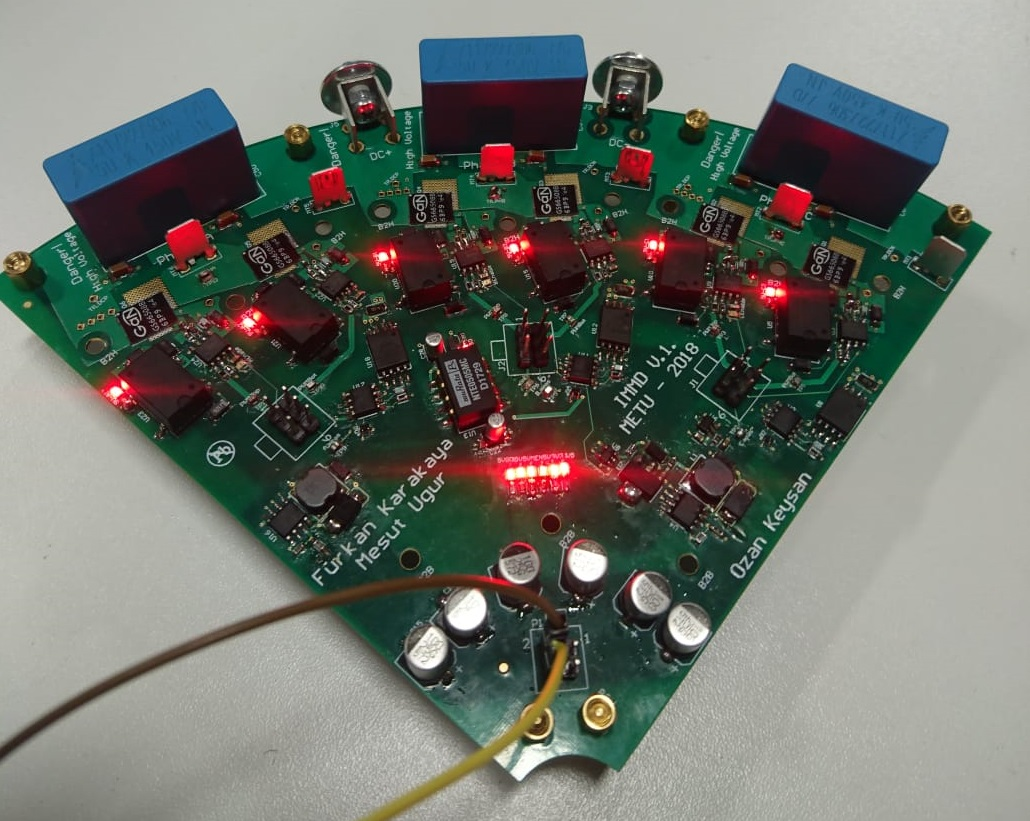
\includegraphics[width=6cm]{figures/invertermodule.jpg}
\caption{2 kW GaN based 3-phase inverter module}
\label{fig:invertermodule}
\end{minipage}%
\begin{minipage}[b]{.6\linewidth}
\centering
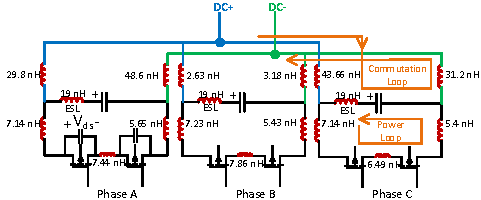
\includegraphics[width=10cm]{figures/SingleModuleInductanceMap.pdf}
\caption{Parasitic Inductance Map of a Single Module}
\label{fig:SingleModuleInductanceMap}
\end{minipage}
\end{figure}

For the inverter circuit given in Fig. \ref{fig:invertermodule}, the power loop and commutation loop inductances are calculated using ANSYS/Q3D finite element analysis tool as given in Fig. \ref{fig:SingleModuleInductanceMap}. The power loop is effective when a switching occurs between top and bottom switches on a half-bridge, and the commutation loop is effective whenever current commutes from one phase to another.

\begin{figure}[tb]
\begin{minipage}[b]{0.6\linewidth}
\centering
\subfloat[\label{fig:SeriesModules}Series]{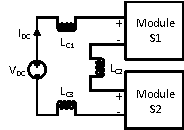
\includegraphics[width=4.5cm]{figures/SeriesModules.pdf}}\quad
\subfloat[\label{fig:ParallelModules}Parallel]{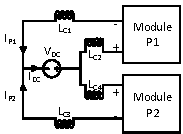
\includegraphics[width=4.5cm]{figures/ParallelModules.pdf}}
\caption{\label{fig:ModuleConnections}Series and Parallel Connected Modules Configurations}
\end{minipage}
\begin{minipage}[b]{0.4\linewidth}
\centering
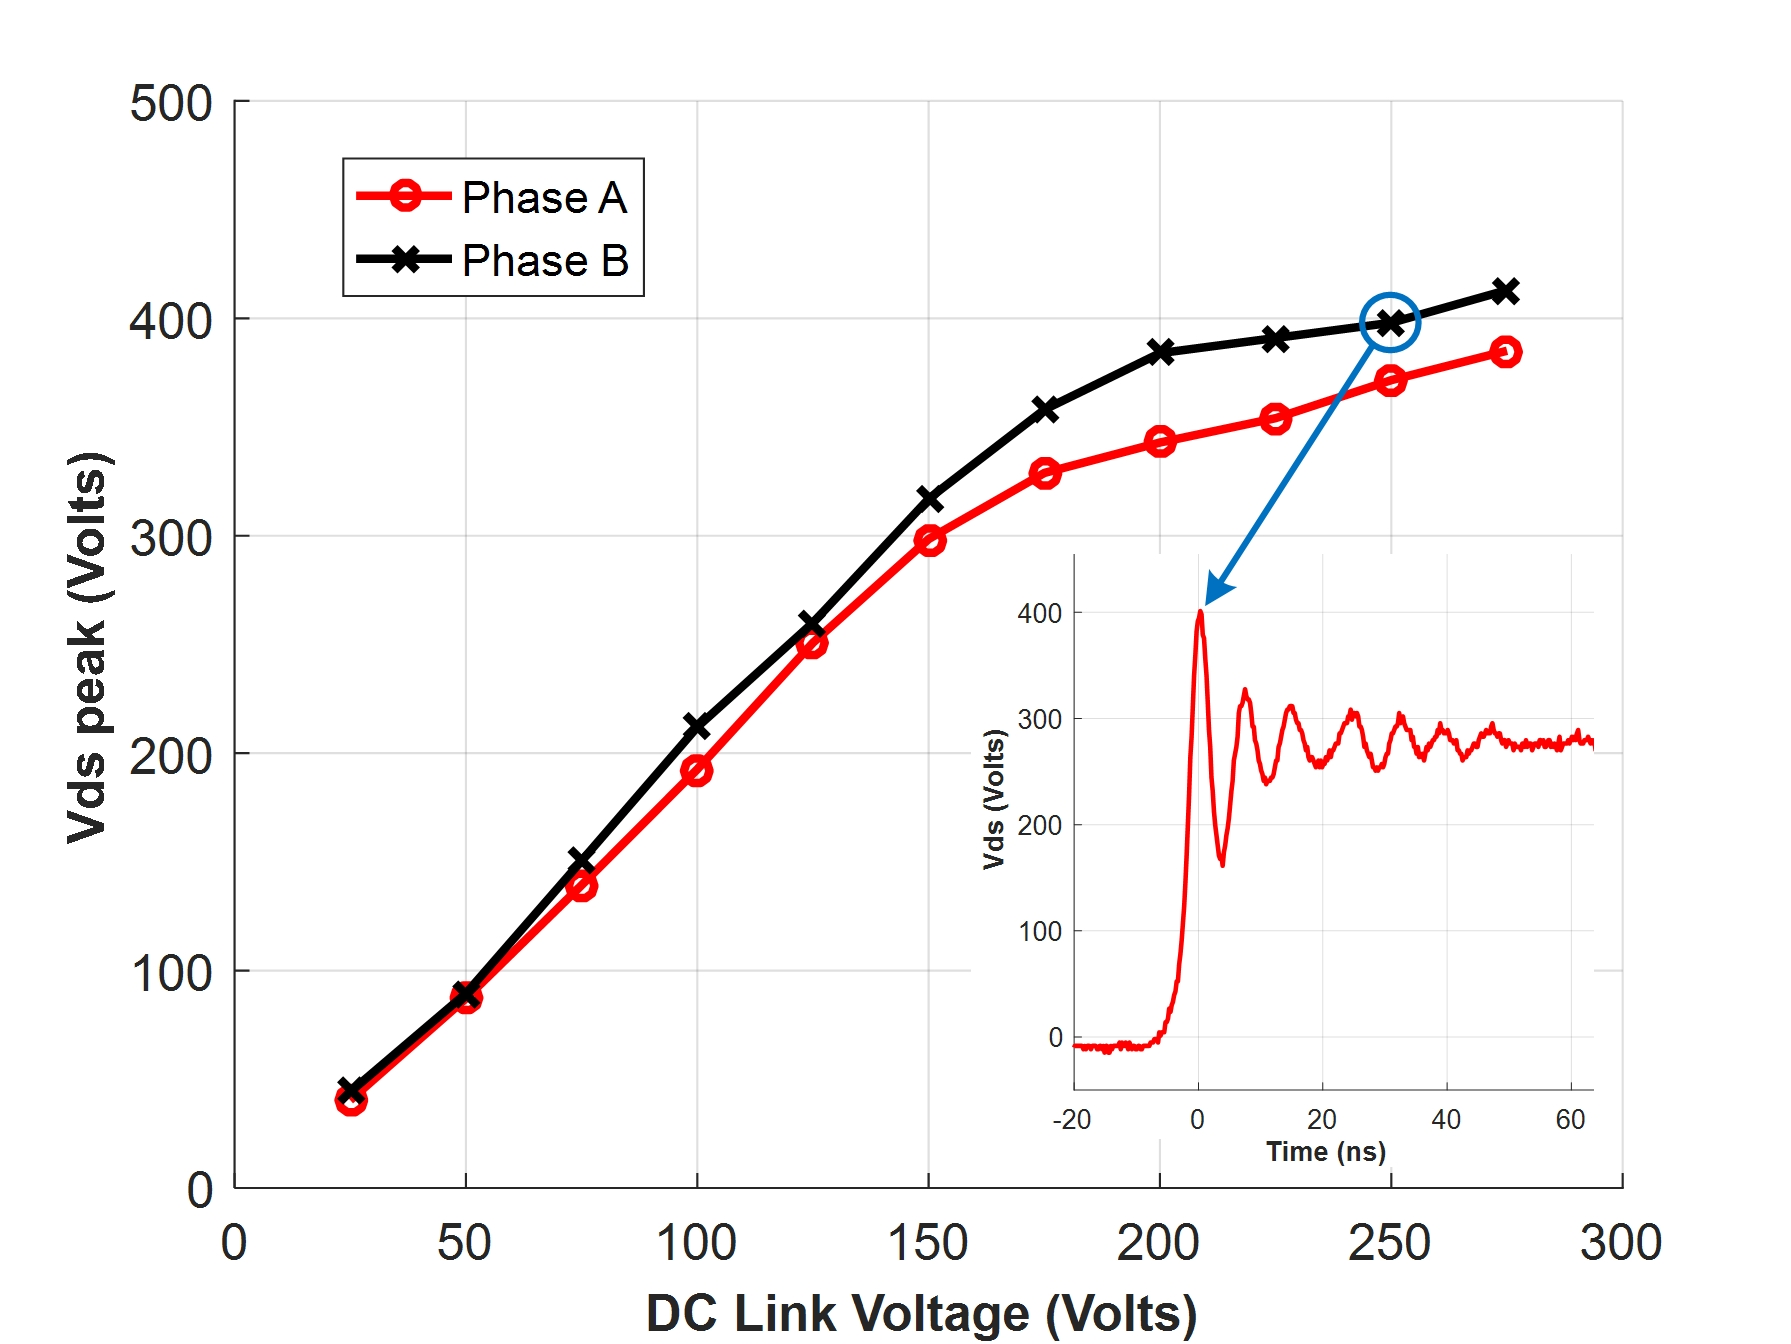
\includegraphics[width=7cm]{figures/experimentalvds2.jpg}
\caption{Experimental voltage overshoot results}
\label{fig:experimentalvds2}
\end{minipage}
\end{figure}

As shown in Fig. \ref{fig:ModuleConnections}, two modules can be connected either in series or in parallel. $L_{C1} \And L_{C3}$, are total equivalent inductances of connectors and module to supply terminal connections and $L_{C2}$ represents the total inductance of the connectors and the module to module connection.
